\section{Result and Discussion}

\subsection{Final Results}
This section presents the results of comparing four optimisation strategies on the ARES Experimental Area beam 
tuning problem, including Nelder-Mead, standard BO, BO\_prior (mismatched), and BO\_prior (matched\_prior\_newtask).  All experiments were run for 100 iterations over 10 independent trials. \

\begin{figure}[ht]
    \centering
    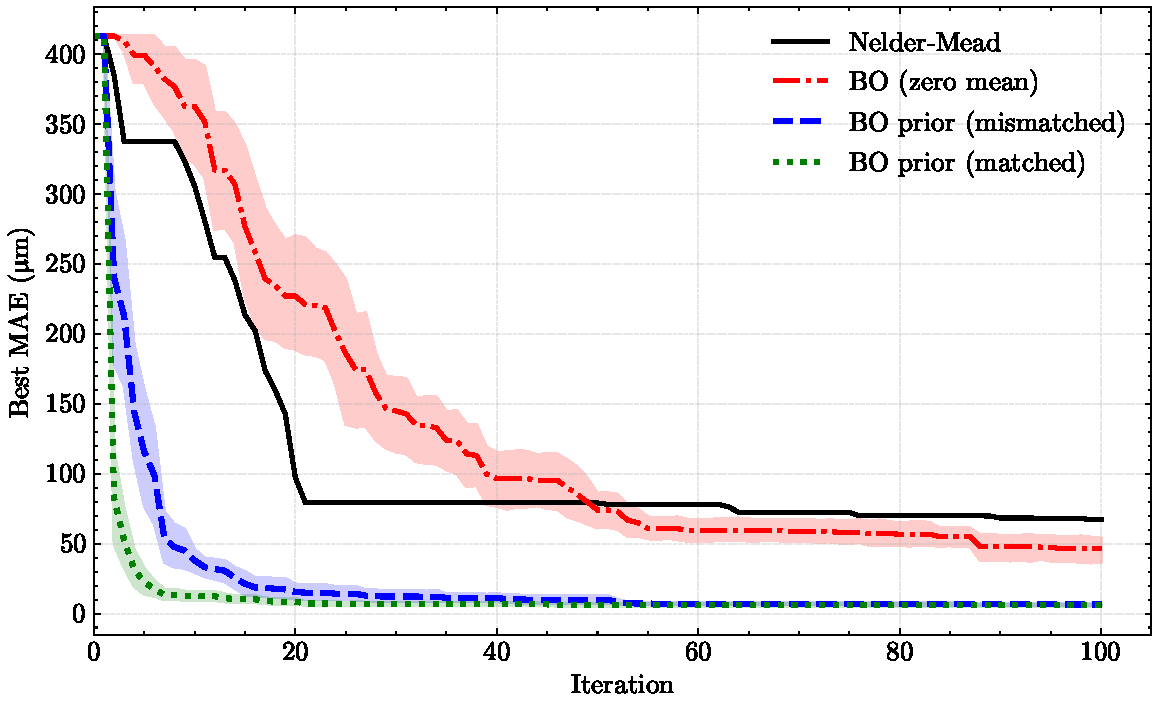
\includegraphics[width=0.8\textwidth]{figures/convergence_curves.pdf}
    \caption{Convergence curve with cumulative minimum MAE over iterations.}
    \label{fig:convergence_curve}
    
\end{figure}

The convergence curves plot in Figure \ref{fig:convergence_curve} highlights the significantly faster convergence of the two physics-informed BO variants compared to the standard BO and Nelder-Mead baselines.
The matched prior (green dotted line) drops sharply within the first 5 iterations, and starts flattening out by iteration 10 already. 
The mismatched prior (blue dashed line) is only slightly behind the matched case which makes sense because the GP needs some observations 
before the optimiser can start correcting the misalignment parameters, thus this case takes roughly 20 iterations to reach a comparable 
level to the matched case. The trajectory of standard BO with zero mean (red dashed-dot line) is more gradual. It does improve 
steadily, but even by iteration 60 , it is still clearly above the physics-informed methods. Additionally, the broad shaded region around, 
indicates more uncertainty in BO standard case, reflecting the fact that without any guidance from prior, 
the initial random exploration phase can either go well or poorly, depending on where the points happen to land. Nelder-Mead (solid black line), in the early phase 
(around iterations 10-20), actually decreases more quickly than standard BO, which is the 
characteristic of the simplex method to make large directed steps once it finds a downhill direction. However, it plateaus around  \SI{65}{\mu}m and then never 
goes lower than that. This shows that NM struggles in this five-dimensional space.

\clearpage
\begin{sidewaystable}
\centering
\caption{Performance Metrics Summary (100 iterations, 10 trials, threshold for steps to target and success rate = \SI{40}{\micro\metre}).}
\label{table:results_main}
\small
\renewcommand{\arraystretch}{1.3}

% table part (a): Error metrics
\vspace{0.5em}
\begin{tabular}{l cc cc cc}
\toprule
 & \multicolumn{2}{c}{\textbf{Best MAE} ($\mu$m)}
 & \multicolumn{2}{c}{\textbf{Final MAE} ($\mu$m)}
 & \multicolumn{2}{c}{\textbf{RMSE} ($\mu$m)} \\
\cmidrule(lr){2-3} \cmidrule(lr){4-5} \cmidrule(lr){6-7}
\textbf{Optimiser} & Median & Mean & Median & Mean & Median & Mean \\
\midrule
Nelder-Mead           & 67.13 & $67.13 \pm 0$       & 67.84  & $67.84 \pm 0$        & 229.20 & $229.20 \pm 0$       \\
BO (zero mean)        & 45.88 & $46.21 \pm 14.70$   & 147.96 & $153.29 \pm 66.66$   & 844.64 & $822.19 \pm 118.14$ \\
BO + prior (mismatch) & 6.71  & $6.49 \pm 1.11$     & 40.54  & $41.71 \pm 16.99$    & 219.90 & $240.16 \pm 65.58$  \\
BO + prior (matched)  & 5.75  & $5.89 \pm 1.06$     & 42.60  & $42.09 \pm 16.90$    & 177.57 & $173.11 \pm 19.34$  \\
\bottomrule
\end{tabular}

\vspace{1.5em}

% table part (b): Improvement and efficiency metrics
\begin{tabular}{l cc cc cc c}
\toprule
 & \multicolumn{2}{c}{\textbf{Improv.\ Best} (\%)}
 & \multicolumn{2}{c}{\textbf{Improv.\ Final} (\%)}
 & \multicolumn{2}{c}{\textbf{Steps to target}}
 & \\
\cmidrule(lr){2-3} \cmidrule(lr){4-5} \cmidrule(lr){6-7}
\textbf{Optimiser} & Median & Mean & Median & Mean & Median & Mean & \textbf{Success rate} \\
\midrule
Nelder-Mead           & 83.74 & $83.74 \pm 0$    & 83.57 & $83.57 \pm 0$      & ---  & ---              & 0\%   \\
BO (zero mean)        & 88.89 & $88.81 \pm 3.56$ & 64.16 & $62.87 \pm 16.15$  & 82.5 & $82.5 \pm 5.5$   & 20\%  \\
BO + prior (mismatch) & 98.37 & $98.43 \pm 0.27$ & 90.18 & $89.90 \pm 4.12$   & 10.5 & $10.8 \pm 4.87$  & 100\% \\
BO + prior (matched)  & 98.61 & $98.57 \pm 0.26$ & 89.68 & $89.81 \pm 4.09$   & 4    & $3.6 \pm 1.28$   & 100\% \\
\bottomrule
\end{tabular}

\end{sidewaystable}
\clearpage

Table \ref{table:results_main} presents the aggregated performance metrics across all four optimisers evaluated over 10 independent trials 
of 100 iterations, with a target threshold of \SI{40}{\mu}m. The results show that both the physics-informed BO variants consistently outperform the baseline 
approaches across every metric. BO with prior (matched and mismatched) achieve median best MAE values of \SI{5.75}{\mu}m and \SI{6.71}{\mu}m respectively, which is approximately 10 times lower 
than Nelder-Mead (\SI{67.13}{\mu}m) and BO zero mean (\SI{45.88}{\mu}m). For both matched and mismatched BO prior variants, their improvement percentage (over best MAE) exceeds 98\% compared to 83.74\% of NM and 88.89\% of standard BO.
While a gap between best and final MAE is observed for all BO methods (most probably due to continued exploration after finding good solutions), even at the final iteration step, both matched and mismatched physics-informed BO variants maintain lower MAE 
of \SI{42.60}{\mu}m and \SI{40.54}{\mu}m respectively than both basline methods, NM (\SI{67.84}{\mu}m) and standard BO (\SI{147.96}{\mu}m). This demonstrates that the physics-informed BO does not only find best solution quickly but also 
maintain better performance throughout the optimisation, even during exploratory phases. 
The RMSE values further confirms the advantage of BO with physics-informed prior, with matched prior achieving
the lowest RMSE of \SI{177.57}{\mu}m reflecting the fact that it starts producing good predictions from the very first steps, followed by the mismatched prior with slightly higher value of \SI{219.90}{\mu}m 
since it spends a few early iterations adjusting its internal model, while standard BO and Nelder-Mead have much higher RMSE values of \SI{844.64}{\mu}m and \SI{229.20}{\mu}m respectively. 
This reflects that comparatively to BO with prior variants, both baseline methods have slower convergence and higher errors during the optimisation process. \

The efficiency metrics of steps to target and success rate are also impressive for physics-informed BO, comparatively to the NM and standard BO. The median steps to reach the target of \SI{40}{\mu}m is just 4 for matched prior and 10.5 for mismached prior, with 100\% success rate for both,
while BO zero mean needs 82.5 steps, showing that it meets the target only on rare occasions with success rate of just 20\%, whereas Nelder-Mead never reaches the target within the 100 steps budget. This metrics summary provides a comprehensive picture of the significant advantage of using a physics-informed prior
in BO for accelerator tuning tasks. 


\begin{figure}[ht]
    \centering
    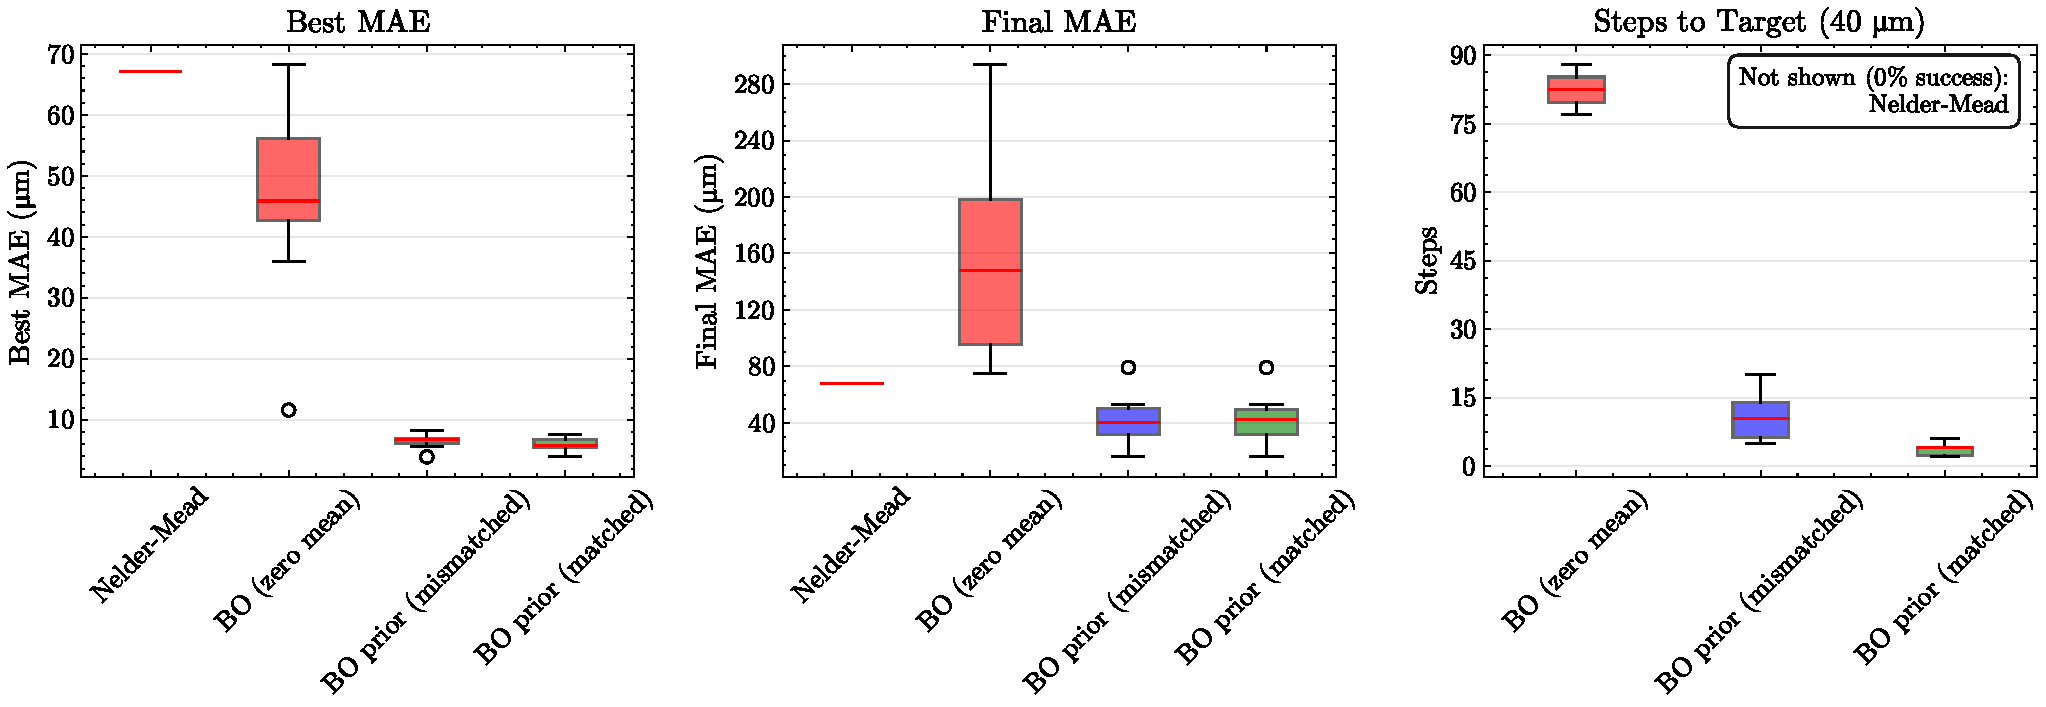
\includegraphics[width=0.8\textwidth]{figures/boxplot_comparison.pdf}
    \caption{Distribution of Best MAE, Final MAE and steps to reach the \SI{40}{\mu}m target across 10 trials for each optimiser.
    the prior-informed BO variants achieve lower error and converge significantly faster than the baseline methods.}
    \label{fig:boxplot_comparison}
    
\end{figure}

The Best MAE panel in Figure \ref{fig:boxplot_comparison} shows that the prior-informed BO variants cluster tightly below \SI{10}{\mu}m in best MAE with minimal spread, whereas the standard BO shows 
high variability (\SI{40}{\mu}m - \SI{56}{\mu}m), while NM consistently converges to same local optimum around \SI{67}{\mu}m. 
The final MAE panel highlights the exploration behavior of BO, where standard BO shows the largest spread (\SI{80}{\mu}m - \SI{280}{\mu}m), yet the prior-informed
BO methods maintain final MAE values around \SI{40}{\mu}m, which is still better than both baseline techniques even at the last iteration. The most striking contrast appears
in the Steps to Target panel, visually confirming that standard BO requires 75-90 steps to reach the target in very few trials,
wheras both BO with prior variants  reach the target within 5-15 steps during the trials, confirming that
prior knowledge significantly accelerates convergence in addition to improving the solution quality.


 
\begin{figure}[ht]
    \centering
    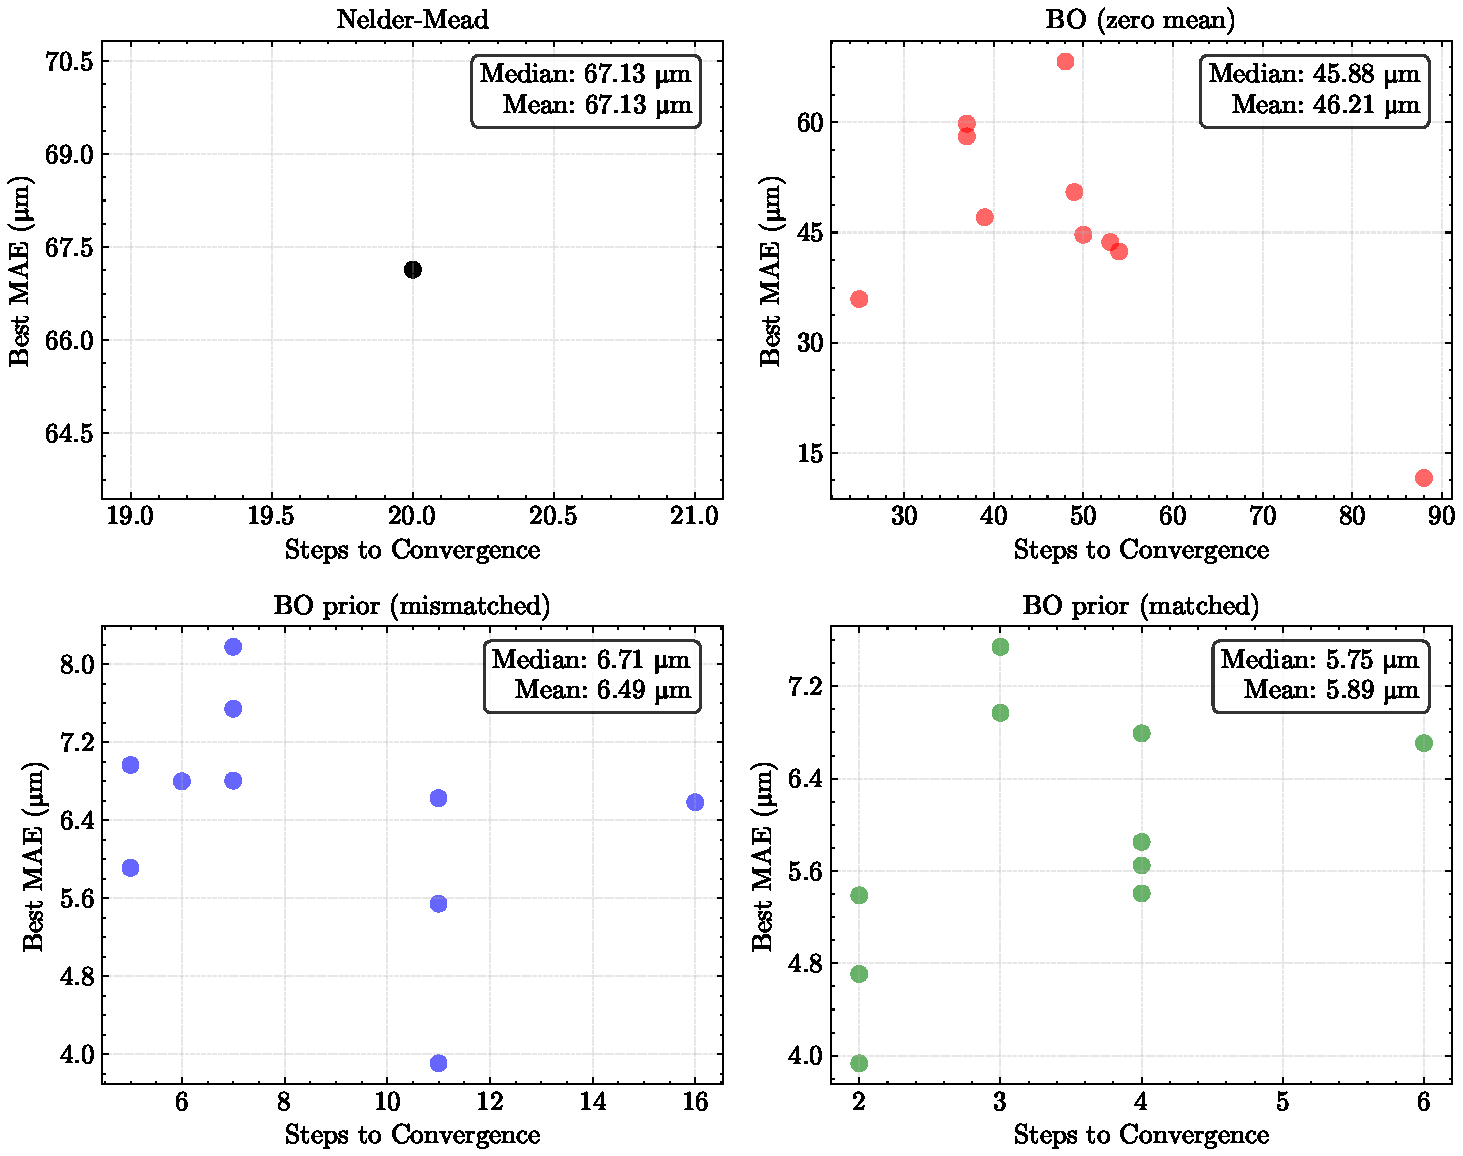
\includegraphics[width=0.8\textwidth]{figures/mae_vs_convergence.pdf}
    \caption{Best MAE vs steps to convergence for each trial, shown per optimiser. 
    Each point represents a single trial, with median and mean Best MAE annotated.}
    \label{fig:scatter_steps_vs_mae}
\end{figure}


The relationship between convergence speed and Best MAE is illustrated by these scatter plots in Figure \ref{fig:scatter_steps_vs_mae}. They provide another perspective by plotting each 
 trials’s Best MAE against how many steps it took to converge. 
NM (black dots) clusters at a single point around step 20, but to a poor solution (approx. \SI{67}{\mu}m).
Standard BO (red dots) shows high variability in both axes, with convergence speed from
25 to 90 steps and Best MAE from 10 to 75 $\mu$m, reflecting inconsistency of optimiser 
without any prior guidane. The prior-informed BO methods occupy the bottom left area of each subplot, which is desirable as
it achieves both low (Best) MAE and fast convergence. BO with matched prior (green dots) takes overall 2-6 steps to converge
with best MAE from 4 to 8 $\mu$m, while BO with mismatched prior (blue dots) takes 5 to 16 steps to a similar quality range as match prior. \


Beyond the aggregate performance metrics, it is worth examining whether the mismatched prior can recover the true quadrupole sets solely from the optimisation data. 
Recalling the ground truth misalignments, the non-zero values were defined in Table \ref{table:misalignment_groundtruth},
while the prior starts with all six values set to zero. By the end of the optimisation process, the optimiser successully adapts and finds
magnet configurations that effectively compensate for the true misalignments, achieving Best MAE values comparabe to the matched prior (\SI{6.71}{\mu}m vs \SI{5.75}{\mu}m). This indicates that BO with mismatched prior is able to leverage the optimisation data to adjust its internal model and effectively learn the true misalignment parameters. Thus, demonstrating robustness to prior mismatch.
This robustness to prior mismatch is a practical significant finding , as exact knowledge of misalignment is rarely available in real accelerator operations.

\subsection{Discussion}
All the results and findings portray a consistent picture that Cheetah-based physics prior delivers a significant improvement 
across every metric, not just in how good the final solution is, but also in how quickly and reliably the optimiser gets there. 
There are several points worth discussing:
\begin{enumerate}
    \item GP is given a warm start by the prior mean function, meaning that its predictions already approximate the shape of the true objective. This means that acquisition functions can make intelligent decisions from very first iterations, rather than going through several steps of  random exploration. The covergence curve plot (Best MAE) makes this especially clear that physics-informed methods are already below 100$\mu$m by 5 iteration steps, but standard BO takes upto iteration 60 or later. Even in the Final MAE case, the physics-informed BO (matched/mismatched) still outperformed at Final step than standard BO and NM. 
    \item One might expect mismatched prior BO to perform significantly worse than matched one due to completely incorrect misalignment values given to it. Whereas, the gap is quite small where the median final errors are almost identical, and the mismatched prior only requires approximately 10 extra steps to attain the 40$\mu$m target (10.5 vs 4). This robustness is encouraged, as real world deployments often involve some degree of mismatch too.
    \item Though standard BO does eventually reach the threshold of \SI{40}{\mu}m with two out of ten trials, but a 20\% success rate and a median Steps to Target of 82.5 are not practical for accelerators where the beam is expensive and operators need reliable tuning within few minutes. While, physics-based approaches (matched + mismatched prior) are able to tackle both concerns.
    \item The fact that Nelder-Mead converges to the same point in every trial (zero standard deviation on the Best and Final errors), indicates its struggle to handle higher-dimensional problems. In a 5-dimensional space with multiple local minima, this is not unexpected from a convex optimisation algorithm. Thus, neither the Best MAE (\SI{67.13}{\mu}m), nor the Final MAE (\SI{67.84}{\mu}m) by NM is considered acceptable in practice, as it exceeds the 40$\mu$m threshold.
    \item Compared to the original FODO demonstration \cite{kaiser2024bridging}, which was a two-dimensional problem with a single learnable parameter, this project work used a five-dimensional landscape with six learnable parameters. Still, the methods with physics-informed prior converged well in approximately 10.5 steps (mismatched prior) or 4 steps (matched prior). This shows that the approach scales reasonably well with the problem dimensionality in this scenario. 
\end{enumerate}


